% Created 2018-04-16 Mon 01:27
\documentclass[a4paper,ngerman,11pt]{scrartcl}
\usepackage[utf8]{inputenc}
\usepackage[T1]{fontenc}
\usepackage{fixltx2e}
\usepackage{graphicx}
\usepackage{longtable}
\usepackage{float}
\usepackage{wrapfig}
\usepackage{rotating}
\usepackage[normalem]{ulem}
\usepackage{amsmath}
\usepackage{textcomp}
\usepackage{marvosym}
\usepackage{wasysym}
\usepackage{amssymb}
\tolerance=1000
\usepackage{natbib}
\usepackage[linktocpage,pdfstartview=FitH,colorlinks,linkcolor=black,
anchorcolor=black,citecolor=black,filecolor=black,menucolor=black,urlcolor=black]{hyperref}
\usepackage{ngerman}
\usepackage{url}
\addtokomafont{disposition}{\rmfamily}
\setcounter{secnumdepth}{0}
\author{Christian Sangvik}
\date{15. April 2018}
\title{Kommentar zu S. Giedions\\"`Die Herrschaft der Mechanisierung"'}
\hypersetup{
  pdfkeywords={},
  pdfsubject={},
  pdfcreator={Emacs 25.3.1 (Org mode 8.2.10)}}
\begin{document}

\maketitle
\noindent
Giedion stellt im Vorwort des Textes die Absicht vor, aufzuzeigen, wie es so
weit kommen konnte, dass in unserer Zeit und Gesellschaft das Denken und Fühlen
von einander gespalten wurde. Er stellt die Vermutung nahe, dass dies durch die
Mechanisierung bedingt zu sein scheint.\cite{Giedion1982} Und diese Mechanisierung
hat möglicherweise weiterreichende Konsequenzen auf unsere Gesellschaft, als wir
annehmen würden. Den Punkt, dass wir durch das Wissen um diese Umstände und
trotzdem mitmachen dabei total abstumpfen ist für mich ein sehr
einleuchtender. Ob man dann in der Konsequenz den zweiten Weltkrieg daraus
herleiten kann ist fraglich, doch zeigt diese gesellschaftliche Haltung
sicherlich grosse Tendenzen in eine zerstörende und selbstzerstörende Richtung.

In den vereinigten Staaten des 19. und 20. Jahrhunderts ist die
Fleischproduktion in eine zuvor unbekannte Masslosigkeit ausgeartet. Begonnen
hat diese Katastrophe mit einer Reihe von Menschen, die die Fleischproduktion
zur Spekulationswirtschaft verwandelt haben, wo es keine ethischen Grundsätze
sondern nur das Gesetz der besten Rendite gibt. Ermöglicht wurde sie dann aber
erst durch den technischen Fortschritt, sowohl in der Produktion wie auch im
Transport, und somit durch die Möglichkeit das Schlachten der Lebewesen am
Fliessband zu erledigen.\cite{Giedion1982} Um die "`Produktion"' zu mechanisieren
wurde der Schlachtungsprozess von dem eines einzelnen Metzgers mit
"`Kreativität"' \cite{Giedion1982} in einzelne, von Maschinen durchführbare
Schritte unterteilt. Diese sind dann mehr oder minder erflogreich gewesen, so
dass man auch heute noch in einer Schlachterei nicht ohne den menschlichen
Metzger auskommt, doch nur mittels dieser Mechanisierung einen so hohen
"`Durchsatz"' erzielen kann.

Die technische Schwierigkeit liegt darin, geplante und konstruierte Maschinen an
die Zufälligkeiten der organischen Natur anzupassen. Und dann in einem zweiten
Schritt, wie bringe ich das Schwein dazu, sich in diese "`Produktionskette"'
einzugliedern?

Giedion beschreibt den Prozess des Verarbeitens vom lebendigen Schwein hin zum
standardisiert gekühlten Konsumprodukt in einem nüchternen Ton. Trotzdem, dass
er sich sehr eng an die Details der Abläufe und Bedürfnisse einer
Grosschlachterei eingeht, und nicht auf die Tiere die dort am Laufmeter getötet
werden, konnte ich den Text kaum lesen. Wenn man die Zahlen anschaut, und sich
statt der nackten Nummern das Bild von derart vielen Tieren vorzustellen
versucht, kommt mindestens mir das Kotzen und ich werde
wehmütig. Sechtzigtausend Tiere am Tag! Mitte des letzten Jahrhunderts, wohl
verstanden, denn ich gehe nicht davon aus, dass sich diese Zahlen nach unten
entwickelt haben. Sechtzigtausend Tiere, von einer Schlachterei alleine!

Die Katastrophe der Produktion ist nicht das grundsätzliche Schlachten der Tiere
und der Fleischkonsum an und für sich, sondern die schiere Zahl, und das
ausarten dieser wie ein Krebsgeschwür, weit über unsere Bedürfnisse heraus. Die
Katastrophe der Ethik und Gesellschaft ist auf der anderen Seite die
Teilnahmslosigkeit. In einer Zeit wo wir das \emph{Glücklichsein} als Ideal geimpft
bekommen und um derartige Umstände wissen, können wir gar nicht anders als, um
unseres Selbstschutzes willen, zu verdrängen. Es ist auch viel einfacher diese
Misstände, und jene, die damit einher gehen, wie zum Beispiel die \emph{Tierhaltung},
zu ignorieren, als sich selber gegenüber eingestehen zu müssen, dass wir alleine
durch unsere Haltung Massenmörder sind. Wenn es nicht mehr darum geht einen
wirklichen Hunger zu stillen, sondern nur darum, wer denn das grösste Steak hat
kann meiner Meinung nach kein gesunder Umgang entstehen. Und dies ist ja
bekanntlich auch nicht nur ein Problem der Fleischproduktion, sondern generell,
sobald etwas im grossen Stil hergestellt wird; von Kleidung über Kosmetika bis
hin zu unseren Luxusgütern.

Wie also können wir derartige Katastrophen gesellschaftlich aushalten? Der
Prozess, der diesem Phänomen zugrunde liegt ist das Anonymisieren. Wir
Verbraucher anonymisieren uns in der Gruppe der gesamten Konsumenten, und der
Metzger in der Grossschlachterei anonymisiert sich in der geteilten Arbeit, wo
er nur einen kleinen Teil des Prozesses ausführt, und nicht mehr dem Tier von
Angesicht zu Angesicht gegenübersteht. Durch diese Anonymisierung fehlt uns der
Bezug zur Katastrophe. Wir haben das faktische Wissen darum, können in unserer
Gefühlswelt aber nichts anfangen damit, da wir uns nicht mehr betroffen
fühlen. Und dies hat sich sicherlich massgeblich durch die Mechanisierung
eingestellt. Denn wenn ich mein Tier, das ich essen will selber herzüchte und
selber schlachten müsste, wäre ich nicht in einer Bezugslosigkeit dazu. Doch für
uns konnt das Fleisch halt aus dem Supermarkt und nicht aus dem eigenen
Stall. Die perversion hierbei liegt natürlich in dem Punkt, dass wir während dem
wir ein Stück Schwein oder Rind essen unsere Katze streicheln. Unsere Haltung
inst nicht eine unemphatische sondern eine selektiv verachtende. Natürlich hat
aber auch die Benennung \emph{Nutztier} hier ihren Beitrag geleistet.

Ich komme nicht umhin das Wort pervers noch einmal zu verwenden, denn ich finde
es einfach krank, dass wir uns sogar gleichzeitig noch einreden, gutes zu tun
für den Planeten auf dem wir zu Gast sind und auf die Umwelt zu schauen, wie wir
aber mittags ein halbes Hänchen für 4 Franken haben müssen. Dass für dieses Geld
keine Ethik dem Tier gegenüber zu erwarten ist, dürfte auf der Hand liegen. Also
sind es eigentlich wir, die diese Katastrophe zu verantworten haben. Wir haben
sie vielleicht nicht verursacht, doch halten wir sie mit unserer Nachfrage am
leben.

\noindent
\begin{figure}[htb]
\centering
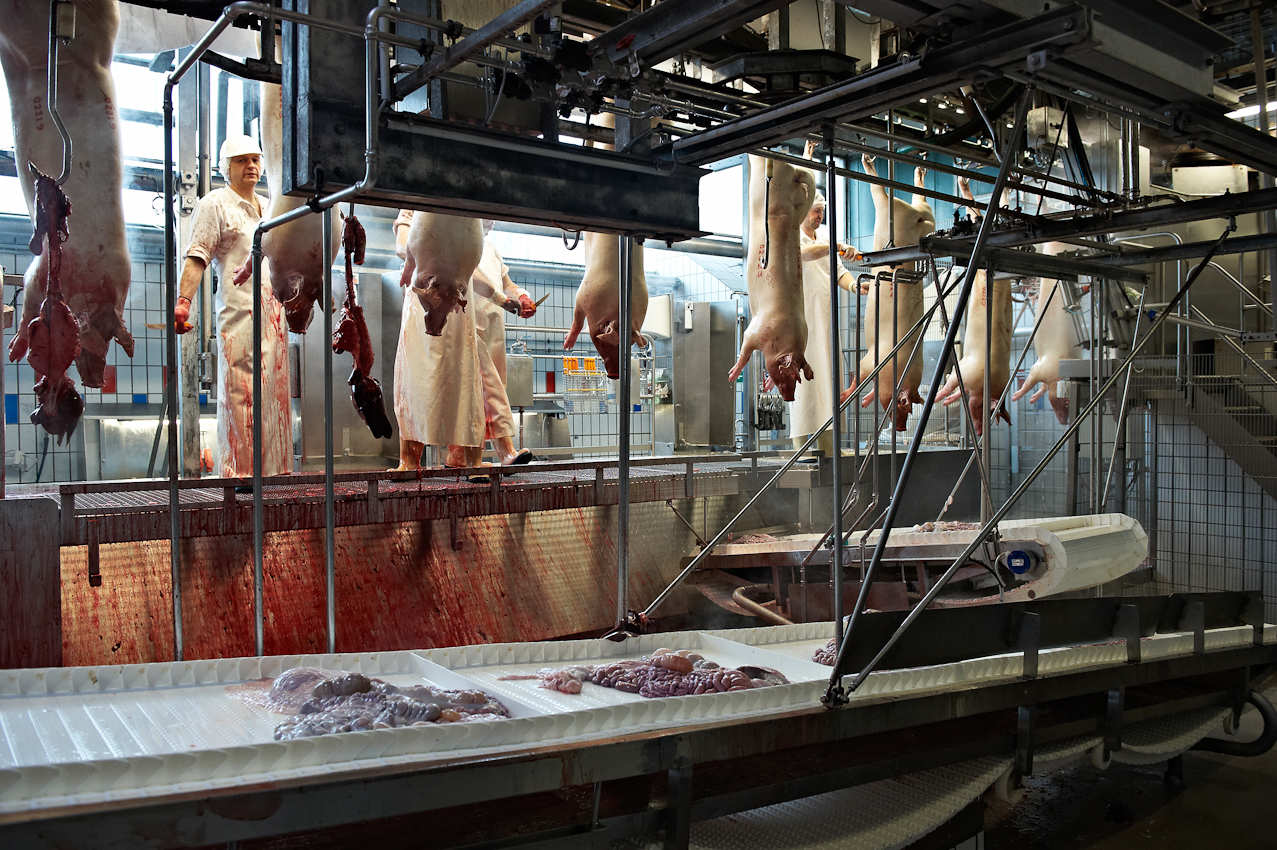
\includegraphics[width=\textwidth]{Bilder/frommann_ronald_02-export.jpg}
\bicaption{}{Akkordarbeit in der lokalen Metzgerei in Luckau, Niedersachsen,\\Bild aufgenommen von Ronald Frommann, 2010\\http://www.eintagdeutschland.de/niedersachsen/schlachthof\\[Eingesehen am 13. April 2018]}
\end{figure}

\noindent
Mein Bild erzählt die Geschichte, dass auch \emph{lokale Schalchtereien} in
Deutschland gemäss der amerikanischen Grossschlachterei funktionieren. Wir
müssen der Tatsache ins Auge sehen, dass auch das Label \emph{lokal} keinen Einfluss
darauf hat, wie es produziert wird, und uns vom romantischen Bild des kleinen
lösen. Denn es scheint es in der Produktion nicht mehr zu geben. Die
Mechanisierung des Schlachtens ist mittlerweile überall. Günstige Arbeiter
verarbeiten jeden Tag Unmengen an Fleisch, damit wir unseren Konsumgewohnheiten
nachgehen können, und sich ein Spekulant und Besitzer einer Schlachterei eine
goldene Nase auf Kosten der Tiere verdient.

\bibliographystyle{unsrt}
\bibliography{Technikgeschichte}
% Emacs 25.3.1 (Org mode 8.2.10)
\end{document}
